\documentclass[12pt]{article}

\usepackage[utf8x]{inputenc} % Включаем поддержку UTF8  
\usepackage[russian]{babel}  % Включаем пакет для поддержки русского языка  
\usepackage{hyperref}        % Для гиперссылок

% Математика
\usepackage{amsmath}         % В т.ч. для матриц
\usepackage{amssymb}

% Прога
\usepackage{etoolbox}
\usepackage{listings}

% Цвета
\usepackage{xcolor}

% Картинки
\usepackage{graphicx}
\graphicspath{ {./images/} }

\newtheorem{property}{Свойство}
\newtheorem{consequence}{Следствие}[property]

\newcommand{\qedsymbol}{\rule{2mm}{2mm}}

\begin{document}

\thispagestyle{empty}
\begin{center}
\textbf{ПРАВИТЕЛЬСТВО РОССИЙСКОЙ ФЕДЕРАЦИИ}

\vspace{5ex}
	
\textbf{Федеральное государственное автономное образовательное учреждение \\ высшего образования \\ <<Национальный исследовательский университет \\ <<Высшая школа экономики>>}
\end{center}
\vspace{5ex}

\begin{center}
    Московский институт электроники и математики им. А.Н. Тихонова  
    
    \vspace{5ex}
    
    Департамент прикладной математики
    
    \vspace{10ex}
    \textbf{Отчёт \\ по лабораторной работе №1 \\ по курсу <<Алгоритмизация и программирование>>}
	\vspace{7ex}

\end{center}

\begin{center} 
\begin{tabular}{| p{0.3\linewidth}| p{0.3\linewidth}| p{0.3\linewidth}|}
 \hline	
ФИО студента & Номер группы & Дата \\  \hline
 & & \\  
Вязов Глеб \newline Дмитриевич & БПМ-231 & 18.09.2023\\  
 & & \\  \hline		
\end{tabular}
\end{center}

\begin{center}
	\vspace{3ex}
	
	\vfill
   
   \normalsize
    
	\textbf{Москва, 2023}
\end{center}

\newpage

%---------------------------------------------------------------------------------

\section*{Задание (вариант №7)}
Даны целые числа x, y и вещественное z. Вычислить a и b.


Используя форматный ввод/вывод, организуйте дружественный интерфейс ввода данных
для решения задачи, а затем выведите на экран значения x, y и z (последнее в экспоненциальной форме с точностью 5 знаков после десятичного разделителя). Каждое значение выводить на новой строке, ширина поля – 10.


Вычисленные значения a и b выведите в десятичном формате с точностью 4 знака после
десятичного разделителя. Целое x отобразите в восьмеричном представлении, а y – в
шестнадцатеричном.

$$a = 
\ln \Bigg| \biggl(y-\sqrt{|x|} \biggr) \biggl(x - \frac{y}{|x| - \frac{x^2}{4}} \biggr) \Bigg|
$$

$$
b = 
x - \frac{x^2}{3!} + \frac{x^5}{5!}
$$

\newpage

%---------------------------------------------------------------------------------

\section*{Решение}\addcontentsline{toc}{section}{Решение}

\lstset{ %
texcl=true,%
language=C,                 % выбор языка для подсветки
basicstyle=\small\sffamily, % размер и начертание шрифта для подсветки кода
numbers=left,               % где поставить нумерацию строк (слева\справа)
numberstyle=\tiny,           % размер шрифта для номеров строк
stepnumber=1,                   % размер шага между двумя номерами строк
numbersep=5pt,                % как далеко отстоят номера строк от подсвечиваемого кода
backgroundcolor=\color{white}, % цвет фона подсветки - используем \usepackage{color}
showspaces=false,            % показывать или нет пробелы специальными отступами
showstringspaces=false,      % показывать или нет пробелы в строках
showtabs=false,             % показывать или нет табуляцию в строках
frame=single,              % рисовать рамку вокруг кода
tabsize=3,                 % размер табуляции по умолчанию равен 2 пробелам
captionpos=t,              % позиция заголовка вверху [t] или внизу [b] 
breaklines=true,           % автоматически переносить строки (да\нет)
breakatwhitespace=false, % переносить строки только если есть пробел
escapeinside={\%*}{*)},   % если нужно добавить комментарии в коде
inputencoding=utf8x,
extendedchars=\true
}

\begin{lstlisting}[label=string_code1,caption=C]
#include <stdio.h>
#include <math.h> // Подключение модуля для работы с математикой

int main() {
    // Меняем кодировку на UTF-8, чтобы можно было писать на русском
    system("chcp 65001");

    int x, y;
    double z, a, b;

    // Ввод переменных. Дружественный интерфейс
    printf("Выполнил задание: Вязов Глеб. Группа: БПМ231\n");
    printf("Введите значение x целое: ");
    scanf("%d", &x);
    printf("Введите значение y целое: ");
    scanf("%d", &y);

    printf("Введите значение z дробное: ");
    scanf("%lf", &z);

    // Считаем значение a
    a = log(fabs(
            (y-sqrt(abs(x)))*
            (x - y / (double) (abs(x) + pow(x, 2) / (double) 4))
            ));

    // Считаем значение b
    b = x - (pow(x, 2) / (double) (1*2*3))
            + (pow(x, 5) / (double) (1*2*3*4*5));

    // Вывод
    printf("\nx =%10d\ny =%10d\nz =%10.5e\n", x, y, z);
    printf("\na =%10.4lf\nb =%10.4lf\n", a, b);

    // Вывод x(8)
    printf("\nx(8) =%o", x);

    // Вывод y(16)
    printf("\ny(16) =%x", y);

    return 0;
}

\end{lstlisting} 

\newpage

%---------------------------------------------------------------------------------

\section*{Тестирование}

\begin{enumerate}

\item \textbf{Тест №1.} 

\textit{Ввод:} 10, 17, 3.14

\textit{Вывод:} 

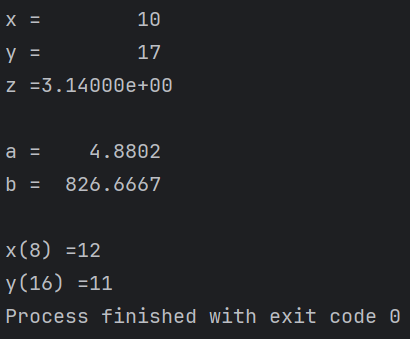
\includegraphics{img1}

\item \textbf{Тест №2.}

\textit{Ввод:} -10, -17, 3.14

\textit{Вывод:} 

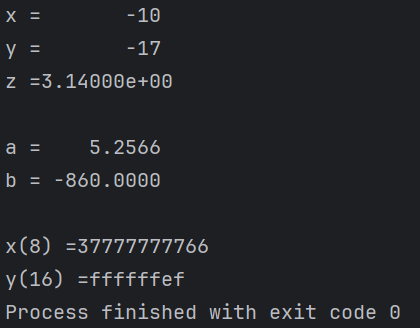
\includegraphics{img2}

\item \textbf{Тест №3.}

\textit{Ввод:} 18, -23, 2.14

\textit{Вывод:} 

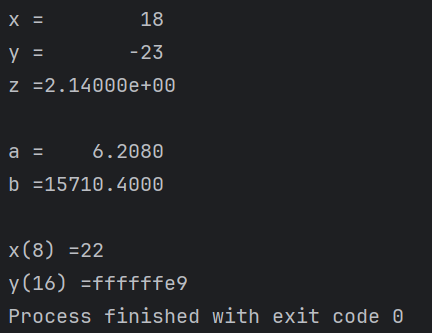
\includegraphics{img3}

\end{enumerate}


\end{document}
